% Based on the author's NKU template; original MIT license retained.
\documentclass[UTF8,notitlepage,11pt]{ctexart}
\usepackage[a4paper,margin=1in]{geometry}
\usepackage{amsmath,graphicx,booktabs,tabularx,array,float,longtable}
\usepackage{fancyhdr,fvextra,enumitem,tikz,xcolor}
\usetikzlibrary{arrows.meta,positioning,shapes.geometric}
\usepackage[colorlinks=true,linkcolor=blue!45!black,urlcolor=blue!55!black]{hyperref}
\usepackage{xurl}
\setlength{\headheight}{15pt}\pagestyle{fancy}\fancyhf{}
\fancyhead[L]{尚文轩 / 2412456}\fancyhead[R]{计算机网络 · 实验三}\fancyfoot[C]{\thepage}
\setlength{\parskip}{4pt}\renewcommand{\arraystretch}{1.18}
\setlist{nosep,topsep=4pt}
\DefineVerbatimEnvironment{code}{Verbatim}{fontsize=\small,frame=single,breaklines=true}
\newcommand{\src}[1]{\nolinkurl{#1}}
\newcommand{\UnitCount}{32}
\newcommand{\IntegrationCount}{20}
\newcommand{\TestTime}{10.421}
\newcommand{\TestTimestamp}{2026-10-22 01:09:19 +0800}
\newcommand{\BenchRuns}{36}
\newcommand{\BenchBytes}{131072}
\newcommand{\BenchTime}{107.282}

\title{\vspace*{-1.2cm}
\includegraphics[width=.95\textwidth]{nankai.jpg}\\[1.2em]
{\bfseries\Huge 实验报告}\\[1em]{\LARGE 实验03：基于UDP服务的可靠传输\\协议设计与编程实现}}
\author{\begin{minipage}{.85\textwidth}\centering\Large
姓名：\underline{尚文轩}\\[.6em]学号：\underline{2412456}\\[.6em]
专业：\underline{计算机科学与技术}\\[.6em]任课教师：\underline{徐敬东、张建忠}\end{minipage}}
\date{\Large 2026年10月22日}
\begin{document}
\maketitle\thispagestyle{empty}\clearpage\pagenumbering{arabic}
{\small\setlength{\parskip}{0pt}\tableofcontents}\clearpage

\section{实验目标与验证范围}
本实验以 UDP 数据报套接字为基础，在用户空间实现面向连接的单向可靠文件传输协议 RUDP-SR/1。
业务数据仅从发送端流向接收端，握手、确认、关闭与异常通知双向交互。程序使用 C++17 和基础 Winsock API，
自行实现连接状态、差错检测、流水线选择确认重传与固定窗口，不使用 CSocket、现成可靠 UDP 或传输框架。

课程《实验说明》第6页强调连接管理、校验和、选择确认、同大小固定窗口，以及在规定环境传输给定文件；第8页要求运行展示、必要日志和传输协议讲解。
该说明及备注中未列出具体文件清单、Router参数或拓扑，因此本报告\textbf{明确采用本机可控模拟链路与自生成文件}。
这不能代替尚未提供的课堂指定环境；同一程序支持任意输入文件、显式地址和端口，可在补充要求后重测。

\begin{table}[H]\centering\small
\caption{实验要求与实现、验证对应}
\begin{tabularx}{\textwidth}{p{.23\textwidth}XX}\toprule
要求 & 实现 & 验证\\\midrule
连接管理 & 建立握手、就绪确认、关闭、TIME\_WAIT、RESET & 各控制报文定点丢失与超时\\
差错检测 & 全首部/正文Internet校验和，整文件CRC32 & 单比特变异、真实损坏、CRC失败\\
流水线与选择确认 & ack\_base + 64位SACK，各段独立计时 & 丢DATA 2时只重传DATA 2\\
同大小固定窗口 & 双方固定W，握手不一致拒绝 & W=1/4/16/64、缓存上界断言\\
单向文件、双向控制 & DATA向接收端，ACK等反向 & 真实UDP进程交互\\
性能与完整交付 & 时间、有效吞吐率、日志、源码、exe、报告 & 36次窗口/丢包实测与SHA256复核\\\bottomrule
\end{tabularx}\end{table}

\section{系统结构与运行环境}
实测使用 Windows 11（10.0.26200）、MSVC 19.29 x64、C++17。
编译参数包含 \src{/W4 /WX /utf-8 /O2 /MT}，警告视为错误并采用静态运行库；链接系统 \src{ws2_32.lib}，运行不依赖 Npcap 或第三方可靠传输库。
Python 仅为测试驱动、数据分析及绘图工具，收发与故障转发均由 C++ 实现。

\begin{figure}[H]\centering
\begin{tikzpicture}[>=Stealth,node distance=11mm,font=\small,
 box/.style={draw,rounded corners,align=center,text width=37mm,minimum height=17mm}]
\node[box] (s) {发送进程\\固定窗口、逐段计时};
\node[box,right=of s] (p) {独立UDP转发器\\丢包、延迟、损坏、重复};
\node[box,right=of p] (r) {接收进程\\乱序缓存、按序写盘};
\draw[->] (s.north east)--node[above]{业务与控制}(p.north west);
\draw[->] (p.north east)--(r.north west);
\draw[<-] (s.south east)--node[below]{确认与关闭}(p.south west);
\draw[<-] (p.south east)--(r.south west);
\end{tikzpicture}\caption{性能实验拓扑；也支持不经过转发器的直接传输}
\end{figure}

转发器使用一个绑定UDP端口双向转发，记住发送端地址，并以实际接收端地址识别返回报文。
它在应用报文上制造差错，不修复 RUDP 校验和；Windows 随后为新的 UDP 数据报计算传输层封装，因此能验证用户空间校验，而非只依赖内核UDP校验。
默认收发仅绑定127.0.0.1；跨主机与外部Router可通过 \src{--bind/--peer/--port/--local-port} 配置。

\section{协议语法与字段定义}\label{sec:wire}
\subsection{基本参数与48字节首部}
每个会话使用非零64位随机ID与对端地址共同标识，避免将其他会话或来源的数据混入当前文件。
固定窗口 $W\in[1,64]$；发送端负载大小 $L$ 默认1200字节，可设为1--1400字节。
最大应用数据报为 $48+1400=1448$ 字节，加IPv4/UDP首部后为1476字节，通常小于1500字节MTU；特殊网络仍应按现场MTU配置。
分段号从0开始，不回绕；
\[
N=\left\lceil\frac{F}{L}\right\rceil\le 2^{32}-1.
\]
空文件的 $N=0$，仍正常建立和关闭。所有多字节字段采用网络字节序，显式序列化，不直接发送C++结构体。

\begin{table}[H]\centering\small\caption{RUDP-SR/1 固定首部}
\begin{tabularx}{\textwidth}{rrlX}\toprule
偏移 & 字节 & 字段 & 语义\\\midrule
0 & 4 & magic & \src{0x52554450}，即RUDP\\
4 & 1 & version & 固定为1\\
5 & 1 & type & 类型1--9\\
6 & 2 & header\_size & 固定为48\\
8 & 8 & session & 非零连接ID\\
16 & 4 & seq & DATA分段号；FIN为总段数；其他为0\\
20 & 4 & ack\_base & 首个未按序提交的分段号\\
24 & 8 & sack & bit i 表示 ack\_base+i 已缓存\\
32 & 2 & payload\_size & 实际数据报长度必须为48加此值\\
34 & 2 & window & 固定窗口W，会话中保持不变\\
36 & 2 & checksum & 首部与正文的16位Internet校验和\\
38 & 2 & reserved & 必须为0\\
40 & 8 & file\_size & 完整文件字节数，与握手一致\\\bottomrule
\end{tabularx}\end{table}

\subsection{消息类型与正文}
\begin{table}[H]\centering\small\caption{消息语义}
\begin{tabularx}{\textwidth}{rlcX}\toprule
值 & 类型 & 方向 & 正文与行为\\\midrule
1 & SYN & S$\to$R & 8字节：chunk(u16)、0(u16)、CRC32(u32)\\
2 & SYN\_ACK & R$\to$S & 回显相同参数，拒绝窗口不一致\\
3 & START & S$\to$R & 相同8字节参数，建立握手末报文\\
4 & DATA & S$\to$R & 分段正文，末段长度按文件大小计算\\
5 & ACK & R$\to$S & 空，使用首部ack\_base与SACK\\
6 & FIN & S$\to$R & CRC32(u32)、总分段数(u32)，seq=N\\
7 & FIN\_ACK & R$\to$S & 空，表示文件已校验并提交\\
8 & CLOSE\_ACK & S$\to$R & 空，确认FIN\_ACK并进入TIME\_WAIT\\
9 & RESET & 双向 & 可读错误原因，会话失败\\\bottomrule
\end{tabularx}\end{table}

除ACK外，ack\_base和sack必须为0；除DATA/FIN外seq必须为0。
\src{SYN/SYN_ACK/START/FIN}正文必须为8字节，\src{ACK/FIN_ACK/CLOSE_ACK}正文必须为空，DATA不能为空。
未知版本、非法长度、保留字段、非法窗口及不符合类型的字段直接丢弃并记录。

\subsection{差错检测}
校验和使用RFC 1071反码求和方法\cite{rfc1071}：将首部及正文按16位大端字相加，奇数末字节补0，折叠高位进位，再按位取反。
构造报文时checksum字段置0后计算；接收时包含checksum求和结果应为全1，即本实现的校验函数返回0。
\begin{code}
while (n >= 2) {
    sum += (uint32_t(p[0]) << 8) | p[1];
    p += 2; n -= 2;
}
if (n) sum += uint32_t(p[0]) << 8;
while (sum >> 16) sum = (sum & 0xffff) + (sum >> 16);
return static_cast<uint16_t>(~sum);
\end{code}
错误报文不发送肯定ACK，由发送端独立超时恢复。接收端按顺序写入时另增量计算整文件CRC32，提交前与握手参数比较。
测试驱动再用SHA256与逐字节比较独立核对。校验和与CRC32均可能碰撞，不能作为身份认证或抗恶意篡改机制。

\section{连接管理与时序}\label{sec:state}
\subsection{建立连接}
建立交互为SYN、SYN\_ACK、START，并增加ACK(base=0)作为就绪确认；因此正常发送DATA前会看到四条控制报文。
接收端只在合法START后建立临时文件；重复SYN或START重发响应，不重置已经收到的数据。
发送端对每个控制阶段按RTO重试，默认RTO150ms、最多40次重试；接收等待/空闲时限默认10000ms。

\begin{figure}[H]\centering
\begin{tikzpicture}[>=Stealth,font=\small,x=1cm,y=1cm]
\node at (0,0) {发送端};\node at (10,0) {接收端};
\draw[dashed] (0,-.3)--(0,-8.2);\draw[dashed] (10,-.3)--(10,-8.2);
\draw[->] (0,-.7)--node[above]{SYN(session,W,F,L,CRC32)}(10,-.7);
\draw[<-] (0,-1.4)--node[above]{SYN\_ACK：参数回显}(10,-1.4);
\draw[->] (0,-2.1)--node[above]{START}(10,-2.1);
\draw[<-] (0,-2.8)--node[above]{ACK(base=0)：接收就绪}(10,-2.8);
\draw[->] (0,-3.5)--node[above]{DATA流水线}(10,-3.5);
\draw[<-] (0,-4.2)--node[above]{ACK(base,SACK)，必要时选择重传}(10,-4.2);
\draw[->] (0,-4.9)--node[above]{FIN(CRC32,N)}(10,-4.9);
\node[align=center] at (7,-5.5) {校验长度/CRC32\\提交目标文件};
\draw[<-] (0,-6.2)--node[above]{FIN\_ACK}(10,-6.2);
\draw[->] (0,-6.9)--node[above]{CLOSE\_ACK}(10,-6.9);
\node[align=center] at (2,-7.6) {TIME\_WAIT：3RTO\\响应重复FIN\_ACK};
\node at (8,-7.6) {关闭已确认};
\end{tikzpicture}\caption{建立、单向数据传输与关闭的正常时序}
\end{figure}

\subsection{关闭与异常}
发送端只有全部数据确认后才能发送FIN。接收端检查总段数、累计字节数和CRC32，刷新并关闭临时文件后将其重命名为最终目标，再发送FIN\_ACK。
FIN或FIN\_ACK丢失时重复FIN/FIN\_ACK不再次写入文件。发送端收到FIN\_ACK后发送CLOSE\_ACK，在3RTO的TIME\_WAIT内对重复FIN\_ACK再次确认。

每个阶段与数据段都有重试预算。连续丢失超过预算、对端RESET、写盘失败或中断均返回非零状态；未提交文件由本进程删除，不覆盖已有目标或既有.part。
如果接收端已提交文件而CLOSE\_ACK持续丢失，接收端可能在关闭确认超时后失败，已验证文件仍保留，日志明确提示。
这体现了有限重试在永久故障下的状态边界，不能承诺双方对最终状态无限可靠地达成一致。

接收端依次经历\src{LISTEN}、\src{SYN_RECEIVED}、\src{ESTABLISHED}、\src{FILE_COMMITTED/LAST_ACK}和\src{CLOSED}。
发送端依次经历\src{SYN_SENT}、\src{ESTABLISHED}、\src{FIN_WAIT}、\src{TIME_WAIT}和\src{CLOSED}。
Ctrl+C只设置停止标志，通过正常栈展开清理资源；不在控制台回调中写文件或操作复杂共享状态。

\section{固定窗口、选择确认与重传}\label{sec:sr}
\subsection{序号空间不变式}
发送端维护最左未确认序号$s$与下一未发送序号$n$，必须满足
\[
s\le n\le s+W.
\]
接收端维护首个未按序提交号$r$，只缓存$[r,r+W)$中的段。每个段只能被按序写入一次。
发送端不能仅根据“当前未确认数量小于W”就继续向前发送：如果左侧有缺口，即使右侧段均已SACK确认，序号窗口也不能越过缺口。
这保证接收窗口的固定空间约束，并通过单元测试和实际最大在途/缓存计数检查。

\subsection{累计确认与位图映射}
ACK中的ack\_base是$r$，表示所有小于$r$的段都已按序写入；bit i 置1表示$r+i$已收到并缓存在接收窗口。
接收端先连续提交可交付前缀，再计算位图，所以bit 0必为0。
发送端据此清除已确认段的计时记录，只在连续确认前缀形成时推进$s$。

例如丢失DATA 2，而3--7已缓存：ack\_base=2，SACK=\src{0x3E}，即位1--5置1，分别对应3--7。
发送端只保留2为未确认；2超时重传后，接收端一次交付2--7，回复ACK(base=8)。
\begin{table}[H]\centering\small
\caption{缺口场景下的选择确认解释}
\begin{tabular}{ccl}\toprule
字段 & 数值 & 含义\\\midrule
ack\_base & 2 & 0、1已按序提交，2尚缺失\\
sack bit 0 & 0 & 分段2未收到\\
sack bits 1--5 & 1 & 分段3--7已缓存，不需重传\\
补齐后的ack\_base & 8 & 0--7全部提交\\\bottomrule
\end{tabular}\end{table}

发送端还验证ack\_base不得超过已发送前沿，SACK不能包含未发送分段、bit 0或超出W的位，避免错误确认导致跳过数据。

\subsection{逐段超时与接收缓存}
每个未确认段保存报文、最近发送时刻、重传次数。只有超过RTO且仍未确认的段才重传；已SACK的乱序段不会因为左侧缺口而被重传。
这是选择重传，不是Go-Back-N。固定RTO使用单调时钟，轮询及Windows调度会带来实际时间粒度，不保证毫秒配置等于精确链路时延。

接收端收到窗口内新段就缓存，随后从$r$开始连续写入；旧段或重复段只重发当前ACK，不能重复写盘。
窗口外但有效的段不缓存，只反馈当前窗口状态。缓存中的SACK段不是崩溃恢复承诺：本协议没有断点续传，进程失效后需要重新建立传输。

\section{实现结构与核心方法}
\begin{table}[H]\centering\small
\caption{模块与关键实现}
\begin{tabularx}{\textwidth}{p{.27\textwidth}X}\toprule
模块 & 职责\\\midrule
wire.hpp & 48字节序列化、Internet校验和、CRC32、报文约束\\
window.hpp & SendWindow确认推进、ReceiveWindow乱序缓存与按序交付\\
platform.hpp & 基础Winsock函数、IPv4地址、参数、UTF-8路径与资源清理\\
transfer.cpp & 发送/接收状态机、控制重试、逐段计时、临时文件提交、统计\\
relay.cpp & 独立双向UDP故障转发，随机与定点故障\\
main.cpp & 命令入口、退出码、最终JSON与统计文件\\
tests/ & 32项协议测试、20项集成测试、36次性能与独立SHA256复核\\\bottomrule
\end{tabularx}\end{table}

\subsection{基础Socket调用}
启动调用WSAStartup，创建 \src{socket(AF_INET,SOCK_DGRAM,IPPROTO_UDP)}，通过bind指定本机地址端口。
每次sendto只发送一个完整RUDP报文；select等待可读事件，recvfrom一次取得一个UDP数据报及来源，之后校验实际长度与首部。
最后closesocket、WSACleanup。项目中用于生命周期的小型资源守卫仅负责释放原始句柄，不替代Socket API或协议实现。

\subsection{发送端算法}
\begin{code}
while (base < total_segments) {
    while (next < total_segments && next < base + W)
        send_new_segment_and_start_its_timer();
    if (valid_ACK_received()) {
        mark_cumulative_prefix_and_SACK_bits();
        erase_acknowledged_timers();
        slide_only_contiguous_confirmed_prefix();
    }
    for (each still_unacknowledged_segment)
        if (its_timer_expired()) retransmit_only_that_segment();
}
\end{code}
源码实际使用有序集合管理未确认序号，并用映射保存未确认报文与独立计时。ACK检查、推进与重传分别由明确函数负责。
发送端预扫描文件得到大小与CRC32，此时间不计入传输指标；实际传输按窗口流式读取，内存不随整个文件大小增长。

\noindent\begin{minipage}{\textwidth}
\subsection{接收端与提交}
\begin{code}
insert_if_inside_receive_window(seq, payload);
while (buffer contains recv_base) {
    write_file_and_update_streaming_CRC(buffer[recv_base]);
    erase_buffered_segment();
    ++recv_base;
}
send_ACK(recv_base, bitmap_of_remaining_buffer);
\end{code}
只有写入成功后才增加recv\_base；写盘失败不会被错误地累计确认。
临时文件用Windows CREATE\_NEW创建，最终使用同目录重命名，不覆盖现有目标；异常析构只清理本进程创建且未提交的临时文件。
UTF-16命令行转UTF-8，再经filesystem路径进入Windows文件API，中文输入/输出文件名已覆盖。
\end{minipage}

\section{功能与可靠性实测}
\subsection{测试方法与覆盖}
测试时间为\TestTimestamp{}，\UnitCount{}项协议/窗口测试与\IntegrationCount{}项真实进程测试全部通过，集成过程耗时\TestTime{}秒。
测试程序驱动真实C++收发进程和C++转发器；另外构造合法/非法对端报文，检查接收端错误路径。
所有预期成功传输比较原文件与目标文件字节，并用SHA256独立核对。

32项测试包含RFC校验向量、奇数字节、CRC标准向量、单比特变异、首部字段边界、序号容量、固定窗口、无效ACK、SACK bit63、乱序交付及随机窗口模型。
20项集成测试覆盖空文件、1字节、1200/1201边界、中英文与全部字节值、1MiB二进制、W64、数据/ACK丢失、损坏、乱序、重复、控制丢失、组合故障、窗口不符、重试耗尽、对端不可达、部分文件超时、CRC失败、来源隔离和既有文件保护。

\begin{table}[H]\centering\small\caption{代表性真实传输/故障场景}
\begin{tabular}{lrrrl}\toprule
场景 & 重传 & 校验失败 & 乱序 & 文件结果 \\ \midrule
空文件 & 0 & 0 & 0 & 一致 \\
1 MiB二进制 & 0 & 0 & 0 & 一致 \\
只丢DATA 2 & 1 & 0 & 5 & 一致 \\
末数据ACK丢失 & 1 & 0 & 0 & 一致 \\
DATA损坏 & 1 & 1 & 2 & 一致 \\
首段延迟 & 0 & 0 & 7 & 一致 \\
重复报文 & 0 & 0 & 0 & 一致 \\
握手/关闭丢失 & 0 & 0 & 0 & 一致 \\
组合随机故障 & 14 & 4 & 49 & 一致 \\
窗口不一致 & 0 & 0 & 0 & 明确失败、无最终文件 \\
全部DATA丢失 & 16 & 0 & 0 & 明确失败、无最终文件 \\
\bottomrule\end{tabular}

\end{table}
“明确失败”是异常路径的预期结果，不是将不完整输出当作成功。部分超时与CRC不符均检查最终文件不存在、.part已清理。

\subsection{选择重传的实际日志}
以下来自2048字节、W=8、chunk=256、只丢DATA 2的真实运行，完整输出另存于evidence/cases。
\VerbatimInput[fontsize=\small,breaklines=true,frame=single]{selective-excerpt.txt}
该次恰好重传一个DATA段，日志与SACK映射一致；不会重传已经缓存的3--7。
首段延后60ms但未丢失的另一场景，实际有7次乱序到达、最大缓存8段，DATA重传为0，说明乱序缓存不等于丢失。

\subsection{控制阶段恢复}
控制故障测试分别丢弃建立阶段的三条握手报文与就绪ACK，以及关闭阶段的\src{FIN}、\src{FIN_ACK}和\src{CLOSE_ACK}，最终双方仍正常关闭。
这覆盖握手末确认丢失及关闭末确认丢失；日志中的control\_retries与DATA重传分开统计，避免将握手重试混入数据重传率。
重传预算耗尽时返回非零状态，对端收到RESET后终止；没有对端时SYN重试也会在预算内结束。

\section{窗口与丢包性能实验}\label{sec:performance}
\subsection{配置、计时与单位}
使用同一份确定性生成的128KiB二进制文件（\BenchBytes{}字节），负载1200字节，总计110段。
固定窗口W=1、4、16、64；转发器对两个方向的每个数据报独立按0\%、10\%、20\%概率丢弃；单向配置延迟8ms，RTO100ms。
每个组合用种子2026、2027、2028运行三次，共\BenchRuns{}次，全部SHA256一致。总执行耗时\BenchTime{}秒，包括进程启动与TIME\_WAIT等，不等于下表单次传输时间。

端到端计时从首条SYN发送前至有效FIN\_ACK到达，包含建立、数据、重传、接收校验与文件提交，不包含发送端CRC预扫描及TIME\_WAIT。
\[
G_{\mathrm{MiB/s}}=\frac{F}{2^{20}T},\qquad
G_{\mathrm{Mbit/s}}=\frac{8F}{10^6T}.
\]
这是有效文件吞吐率，不包含首部与重复报文的线速。表中平均吞吐率是三次各自吞吐率的算术平均，不是平均时间的倒数。
转发器的配置延迟不等于精确物理RTT，Windows定时与调度、文件刷新和本机负载都会影响结果。不同窗口虽使用相同种子，但报文到达顺序不同，因此不承诺丢失同一组序号。

\subsection{实测表与图}
\begin{table}[H]\centering\small\caption{固定窗口与双向逐报文丢包概率；每格3次}
\begin{tabular}{rrrrrr}\toprule
丢包概率 & 窗口 & 平均时间/s & 平均MiB/s & MiB/s范围 & 平均重传 \\ \midrule
0\% & 1 & 3.538 & 0.0353 & 0.0352--0.0355 & 0.0 \\
0\% & 4 & 0.966 & 0.1294 & 0.1286--0.1308 & 0.0 \\
0\% & 16 & 0.323 & 0.3866 & 0.3832--0.3887 & 0.0 \\
0\% & 64 & 0.156 & 0.7997 & 0.7824--0.8321 & 0.0 \\
10\% & 1 & 6.160 & 0.0203 & 0.0191--0.0212 & 23.3 \\
10\% & 4 & 2.006 & 0.0627 & 0.0570--0.0691 & 12.3 \\
10\% & 16 & 0.932 & 0.1348 & 0.1268--0.1474 & 12.0 \\
10\% & 64 & 0.450 & 0.2805 & 0.2575--0.3205 & 9.3 \\
20\% & 1 & 10.829 & 0.0116 & 0.0105--0.0127 & 66.0 \\
20\% & 4 & 3.684 & 0.0344 & 0.0304--0.0404 & 41.3 \\
20\% & 16 & 1.372 & 0.0918 & 0.0851--0.1035 & 28.7 \\
20\% & 64 & 0.785 & 0.1740 & 0.1095--0.2087 & 24.0 \\
\bottomrule\end{tabular}

\end{table}
原始36行数据在 \src{evidence/performance.csv}，每次的收发端与转发器统计保存在benchmark子目录，包含SHA256、重传和窗口上界。

\begin{figure}[H]\centering
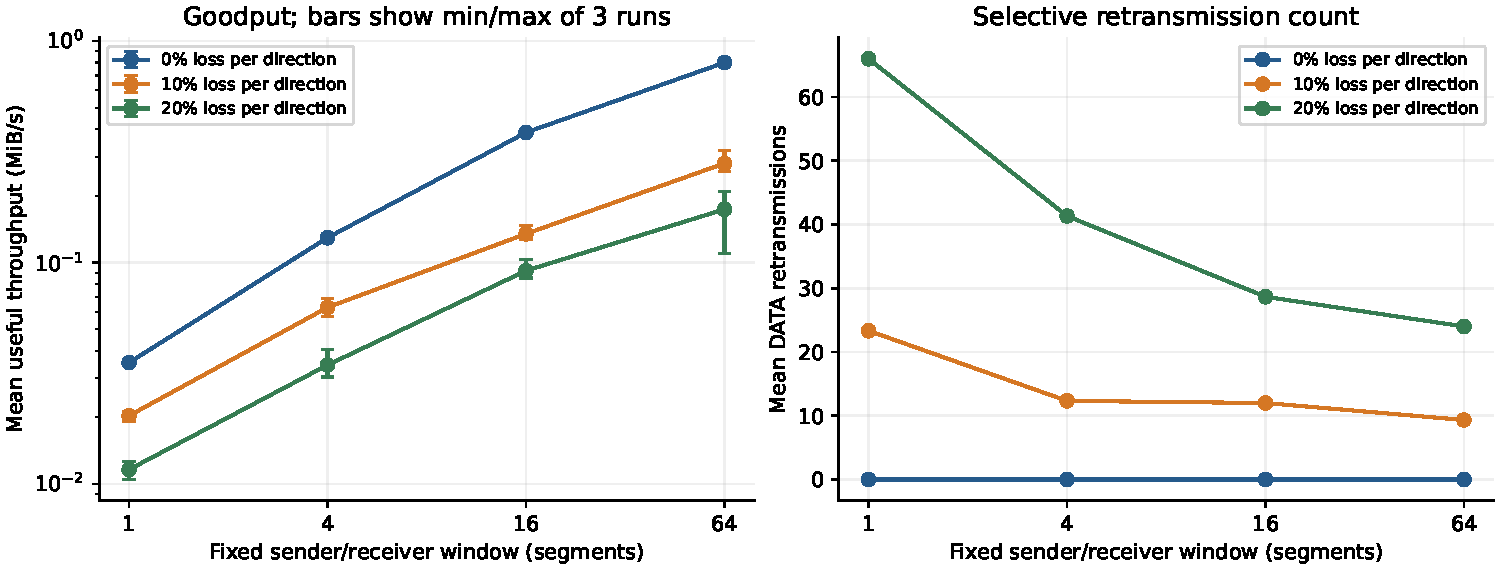
\includegraphics[width=\textwidth]{window-performance.pdf}
\caption{平均有效吞吐率与DATA重传次数；吞吐率误差条表示3次观测的最小/最大值，并非置信区间}
\end{figure}

\subsection{结果解释与局限}
无人工丢包时，W=1的平均有效吞吐率为0.0353MiB/s，W=64为0.7997MiB/s，约提高22.6倍。
20\%逐报文丢包时分别为0.0116与0.1740MiB/s，约提高15倍。W=1相当于停等，增大窗口使多段同时在途，提高等待确认期间的利用率。

同一窗口下丢包增加会降低吞吐率并增加重传；ACK也可能丢失，因此“配置20\%丢包”不能直接等同于20\%DATA重传。
较大窗口允许后续段先收到并SACK确认，缺口恢复后可连续提交；ACK的累计覆盖还可能使个别ACK丢失无需重传数据。
收益不是与W严格线性：握手、文件刷新、定时调度、重试及有限文件长度都带来固定开销。

W64、20\%组的吞吐范围约0.1095--0.2087MiB/s，波动明显，控制报文丢失也会影响总时间。
每组只有3次，本次结果可用于说明窗口影响，不能宣称统计显著或外推到任意真实广域网。
本协议没有拥塞控制，窗口增大不代表在共享网络上可以无限提升发送速率；现场仍应按课堂规定环境重测。

\section{问题处理与结论}
\begin{enumerate}
\item \textbf{UDP不提供连接状态。} 用显式会话ID、地址检查、状态机、幂等重试和RESET建立应用层连接管理。
\item \textbf{仅累计确认无法表达缓存的乱序段。} 增加64位SACK，按ack\_base相对序号映射，逐段停止计时。
\item \textbf{只按未确认数量开窗可能越界。} 以最左缺口和下一序号之差限制固定序号空间，而非仅看容器大小。
\item \textbf{收到不等于完整交付。} 窗口内缓存，按序写入，再做长度和整文件CRC验证；提交前保留.part状态。
\item \textbf{丢失关闭确认可能造成状态分歧。} FIN幂等处理、FIN\_ACK重发、发送TIME\_WAIT；超过预算明确说明最终文件与关闭确认状态。
\item \textbf{性能数值容易口径混乱。} 分清端到端、数据阶段、预扫描与TIME\_WAIT，保留原始三次值、统一MiB/s单位。
\end{enumerate}

本实验完成基于基础UDP套接字的单向可靠文件传输：连接管理、全报文差错检测、流水线选择确认、逐段重传与同大小固定窗口均已实现。
\UnitCount{}项协议测试、\IntegrationCount{}项集成测试和\BenchRuns{}次性能传输提供了可复核证据。
协议边界包括有限重试、无身份认证/加密、无拥塞控制和无断点续传；本机模拟结果与课堂待指定环境明确区分。

\addcontentsline{toc}{section}{参考文献}
\begin{thebibliography}{9}
\bibitem{rfc1071} Braden R., Borman D., Partridge C. Computing the Internet Checksum. RFC 1071, 1988.
\url{https://www.rfc-editor.org/rfc/rfc1071}.
\bibitem{winsock} Microsoft. Using Winsock.
\url{https://learn.microsoft.com/en-us/windows/win32/winsock/using-winsock}.
\bibitem{course} 课程教学材料：《实验说明》，编程实验3与演示讲解要求，第6、8页。2026年课程提供版本。
\end{thebibliography}
\end{document}
